%% abtex2-modelo-artigo.tex, v-1.9.6 laurocesar
%% Copyright 2012-2016 by abnTeX2 group at http://www.abntex.net.br/ 
%%
%% This work may be distributed and/or modified under the
%% conditions of the LaTeX Project Public License, either version 1.3
%% of this license or (at your option) any later version.
%% The latest version of this license is in
%%   http://www.latex-project.org/lppl.txt
%% and version 1.3 or later is part of all distributions of LaTeX
%% version 2005/12/01 or later.
%%
%% This work has the LPPL maintenance status `maintained'.
%% 
%% The Current Maintainer of this work is the abnTeX2 team, led
%% by Lauro César Araujo. Further information are available on 
%% http://www.abntex.net.br/
%%
%% This work consists of the files abntex2-modelo-artigo.tex and
%% abntex2-modelo-references.bib
%%

% ------------------------------------------------------------------------
% ------------------------------------------------------------------------
% abnTeX2: Modelo de Artigo Acadêmico em conformidade com
% ABNT NBR 6022:2003: Informação e documentação - Artigo em publicação 
% periódica científica impressa - Apresentação
% ------------------------------------------------------------------------
% ------------------------------------------------------------------------

\documentclass[
    % -- opções da classe memoir --
    article,            % indica que é um artigo acadêmico
    11pt,               % tamanho da fonte
    oneside,            % para impressão apenas no recto. Oposto a twoside
    a4paper,            % tamanho do papel. 
    % -- opções da classe abntex2 --
    %chapter=TITLE,     % títulos de capítulos convertidos em letras maiúsculas
    %section=TITLE,     % títulos de seções convertidos em letras maiúsculas
    %subsection=TITLE,  % títulos de subseções convertidos em letras maiúsculas
    %subsubsection=TITLE % títulos de subsubseções convertidos em letras maiúsculas
    % -- opções do pacote babel --
    english,            % idioma adicional para hifenização
    brazil,             % o último idioma é o principal do documento
    sumario=tradicional,
    ]{abntex2}


% ---
% PACOTES
% ---

% ---
% Pacotes fundamentais 
% ---
\usepackage{lmodern}            % Usa a fonte Latin Modern
\usepackage[T1]{fontenc}        % Selecao de codigos de fonte.
\usepackage[utf8]{inputenc}     % Codificacao do documento (conversão automática dos acentos)
\usepackage{indentfirst}        % Indenta o primeiro parágrafo de cada seção.
\usepackage{nomencl}            % Lista de simbolos
\usepackage{color}              % Controle das cores
\usepackage{graphicx}           % Inclusão de gráficos
\usepackage{microtype}          % para melhorias de justificação
% ---
        
% ---
% Pacotes adicionais, usados apenas no âmbito do Modelo Canônico do abnteX2
% ---
\usepackage{lipsum}             % para geração de dummy text
\usepackage{fancyvrb}
\usepackage{todonotes}
\usepackage{float}

% ---
        
% ---
% Pacotes de citações
% ---
\usepackage[brazilian,hyperpageref]{backref}     % Paginas com as citações na bibl
\usepackage[alf]{abntex2cite}   % Citações padrão ABNT
% ---

% ---
% Configurações do pacote backref
% Usado sem a opção hyperpageref de backref
\renewcommand{\backrefpagesname}{Citado na(s) página(s):~}
% Texto padrão antes do número das páginas
\renewcommand{\backref}{}
% Define os textos da citação
\renewcommand*{\backrefalt}[4]{
    \ifcase #1 %
        Nenhuma citação no texto.%
    \or
        Citado na página #2.%
    \else
        Citado #1 vezes nas páginas #2.%
    \fi}%
% ---

% ---
% Informações de dados para CAPA e FOLHA DE ROSTO
% ---
\titulo{INE5429 - Segurança em Computação\\ 
        Trabalho Individual 01 - Capitulo 03}
\autor{Bruno Marques do Nascimento\thanks{brunomn95@gmail.com \hspace{1mm} - \hspace{1mm} Universidade Federal de Santa Catarina}}
\instituicao{Universidade Federal de Santa Catarina}
\local{Florianópolis - SC, Brasil}
\data{24 de Março de 2018}
% ---

% ---
% Configurações de aparência do PDF final

% alterando o aspecto da cor azul
\definecolor{blue}{RGB}{41,5,195}

% informações do PDF
\makeatletter
\hypersetup{
        %pagebackref=true,
        pdftitle={\@title}, 
        pdfauthor={\@author},
        pdfsubject={Modelo de artigo científico com abnTeX2},
        pdfcreator={LaTeX with abnTeX2},
        pdfkeywords={abnt}{latex}{abntex}{abntex2}{atigo científico}, 
        colorlinks=true,            % false: boxed links; true: colored links
        linkcolor=blue,             % color of internal links
        citecolor=blue,             % color of links to bibliography
        filecolor=magenta,              % color of file links
        urlcolor=blue,
        bookmarksdepth=4
}
\makeatother
% --- 

% ---
% compila o indice
% ---
\makeindex
% ---

% ---
% Altera as margens padrões
% ---
\setlrmarginsandblock{3cm}{3cm}{*}
\setulmarginsandblock{3cm}{3cm}{*}
\checkandfixthelayout
% ---

% --- 
% Espaçamentos entre linhas e parágrafos 
% --- 

% O tamanho do parágrafo é dado por:
\setlength{\parindent}{1.3cm}

% Controle do espaçamento entre um parágrafo e outro:
\setlength{\parskip}{0.2cm}  % tente também \onelineskip

% Espaçamento simples
\SingleSpacing

% ----
% Início do documento
% ----
\begin{document}

% Seleciona o idioma do documento (conforme pacotes do babel)
%\selectlanguage{english}
\selectlanguage{brazil}

% Retira espaço extra obsoleto entre as frases.
\frenchspacing 

% ----------------------------------------------------------
% ELEMENTOS PRÉ-TEXTUAIS
% ----------------------------------------------------------

%---
%
% Se desejar escrever o artigo em duas colunas, descomente a linha abaixo
% e a linha com o texto ``FIM DE ARTIGO EM DUAS COLUNAS''.
% \twocolumn[           % INICIO DE ARTIGO EM DUAS COLUNAS
%
%---
% página de titulo

\maketitle


% resumo em português
\begin{resumoumacoluna}
    Este documento é referente ao primeiro trabalho individual da disciplina INE5429 - Segurança em computação, com o objetivo de responder algumas questões do capítulo 3 do livro texto da disciplina. Este documento visa responder as perguntas elencadas pelo professor ministrante da disciplina Ricardo Felipe Custódio na plataforma moodle.
 
 \vspace{\onelineskip}
 
\end{resumoumacoluna}

% ]                 % FIM DE ARTIGO EM DUAS COLUNAS
% ---

% ----------------------------------------------------------
% ELEMENTOS TEXTUAIS
% ----------------------------------------------------------
\textual

% ----------------------------------------------------------
% Introdução
% ----------------------------------------------------------
% \section*{Introdução}
% \addcontentsline{toc}{section}{Introdução}

\section*{\textbf{Questões e respostas:}}
\addcontentsline{toc}{section}{Questões e respostas:}


% ----------------------------------------------------------
% Questão 1
% ----------------------------------------------------------
\subsection*{\textbf{3.7 - Show that DES decryption is, in fact, the inverse of DES encryption.}}
\addcontentsline{toc}{subsection}{Questão 3.7}

O DES faz uso do Cifrador de Feistel o qual é provado que seu processo de cifragem é o inverso do de descifragem, como pode ser visto na figura 3.3 de \cite{Stallings:2005:CNS:1076613}. Para o DES precisamos nos atentar as modificações que são realizadas externamente ao cifrador de Feistel utilizado, que são o uso da tabela IP e IP\textsuperscript{-1} e o uso do \texttt{Swap 32 bits}. Por definição a tabela IP\textsuperscript{-1} é a inversa da IP, logo um texto cifrado teve como últimas modificações um \texttt{swap de 32 bits} e sua permutação pela tabela IP\textsuperscript{-1}, logo para decifrá-lo é necessário realizar a operação inversa para gerar o valores corretos de entrada para o cifrador de Feistel. Para desfazer a permutação realizada por IP\textsuperscript{-1} é necessário passar o texto cifrado por uma permutação por IP e depois por um \texttt{swap de 32 bits} que é por si só o inverso de outro \texttt{swap de 32bits} para um entrada de 64 bits. Ao final das rodadas do cifrador de Feistel no processo de decifragem do DES é então necessário desfazer a permutação realizada no processo de cifragem do texto através da tabela IP, para realizar a operação inversa uitliza-se a tabela IP\textsuperscript{-1}, para então obter o texto original. Desta maneira, é mostrado que o processo de decifragem do DES é de fato o processo inverso de cifragem do mesmo. 

% ----------------------------------------------------------
% Questão 2
% ----------------------------------------------------------
\subsection*{\textbf{3.9 - Consider the substitution defined by row 1 of S-box S\textsubscript{1} in Table S.2. Show a block diagram similar to Figure 3.2 that corresponds to this substitution.}}
\addcontentsline{toc}{subsection}{Questão 3.9}

O apêndice S e a tabela S.2 não foram localizados, para responder esta questão foi utilizada como referência a S-box S\textsubscript{1} apresentada nos slides passados em aula.

\begin{figure}[H]
    \label{fig_diagram}
    \begin{center}
        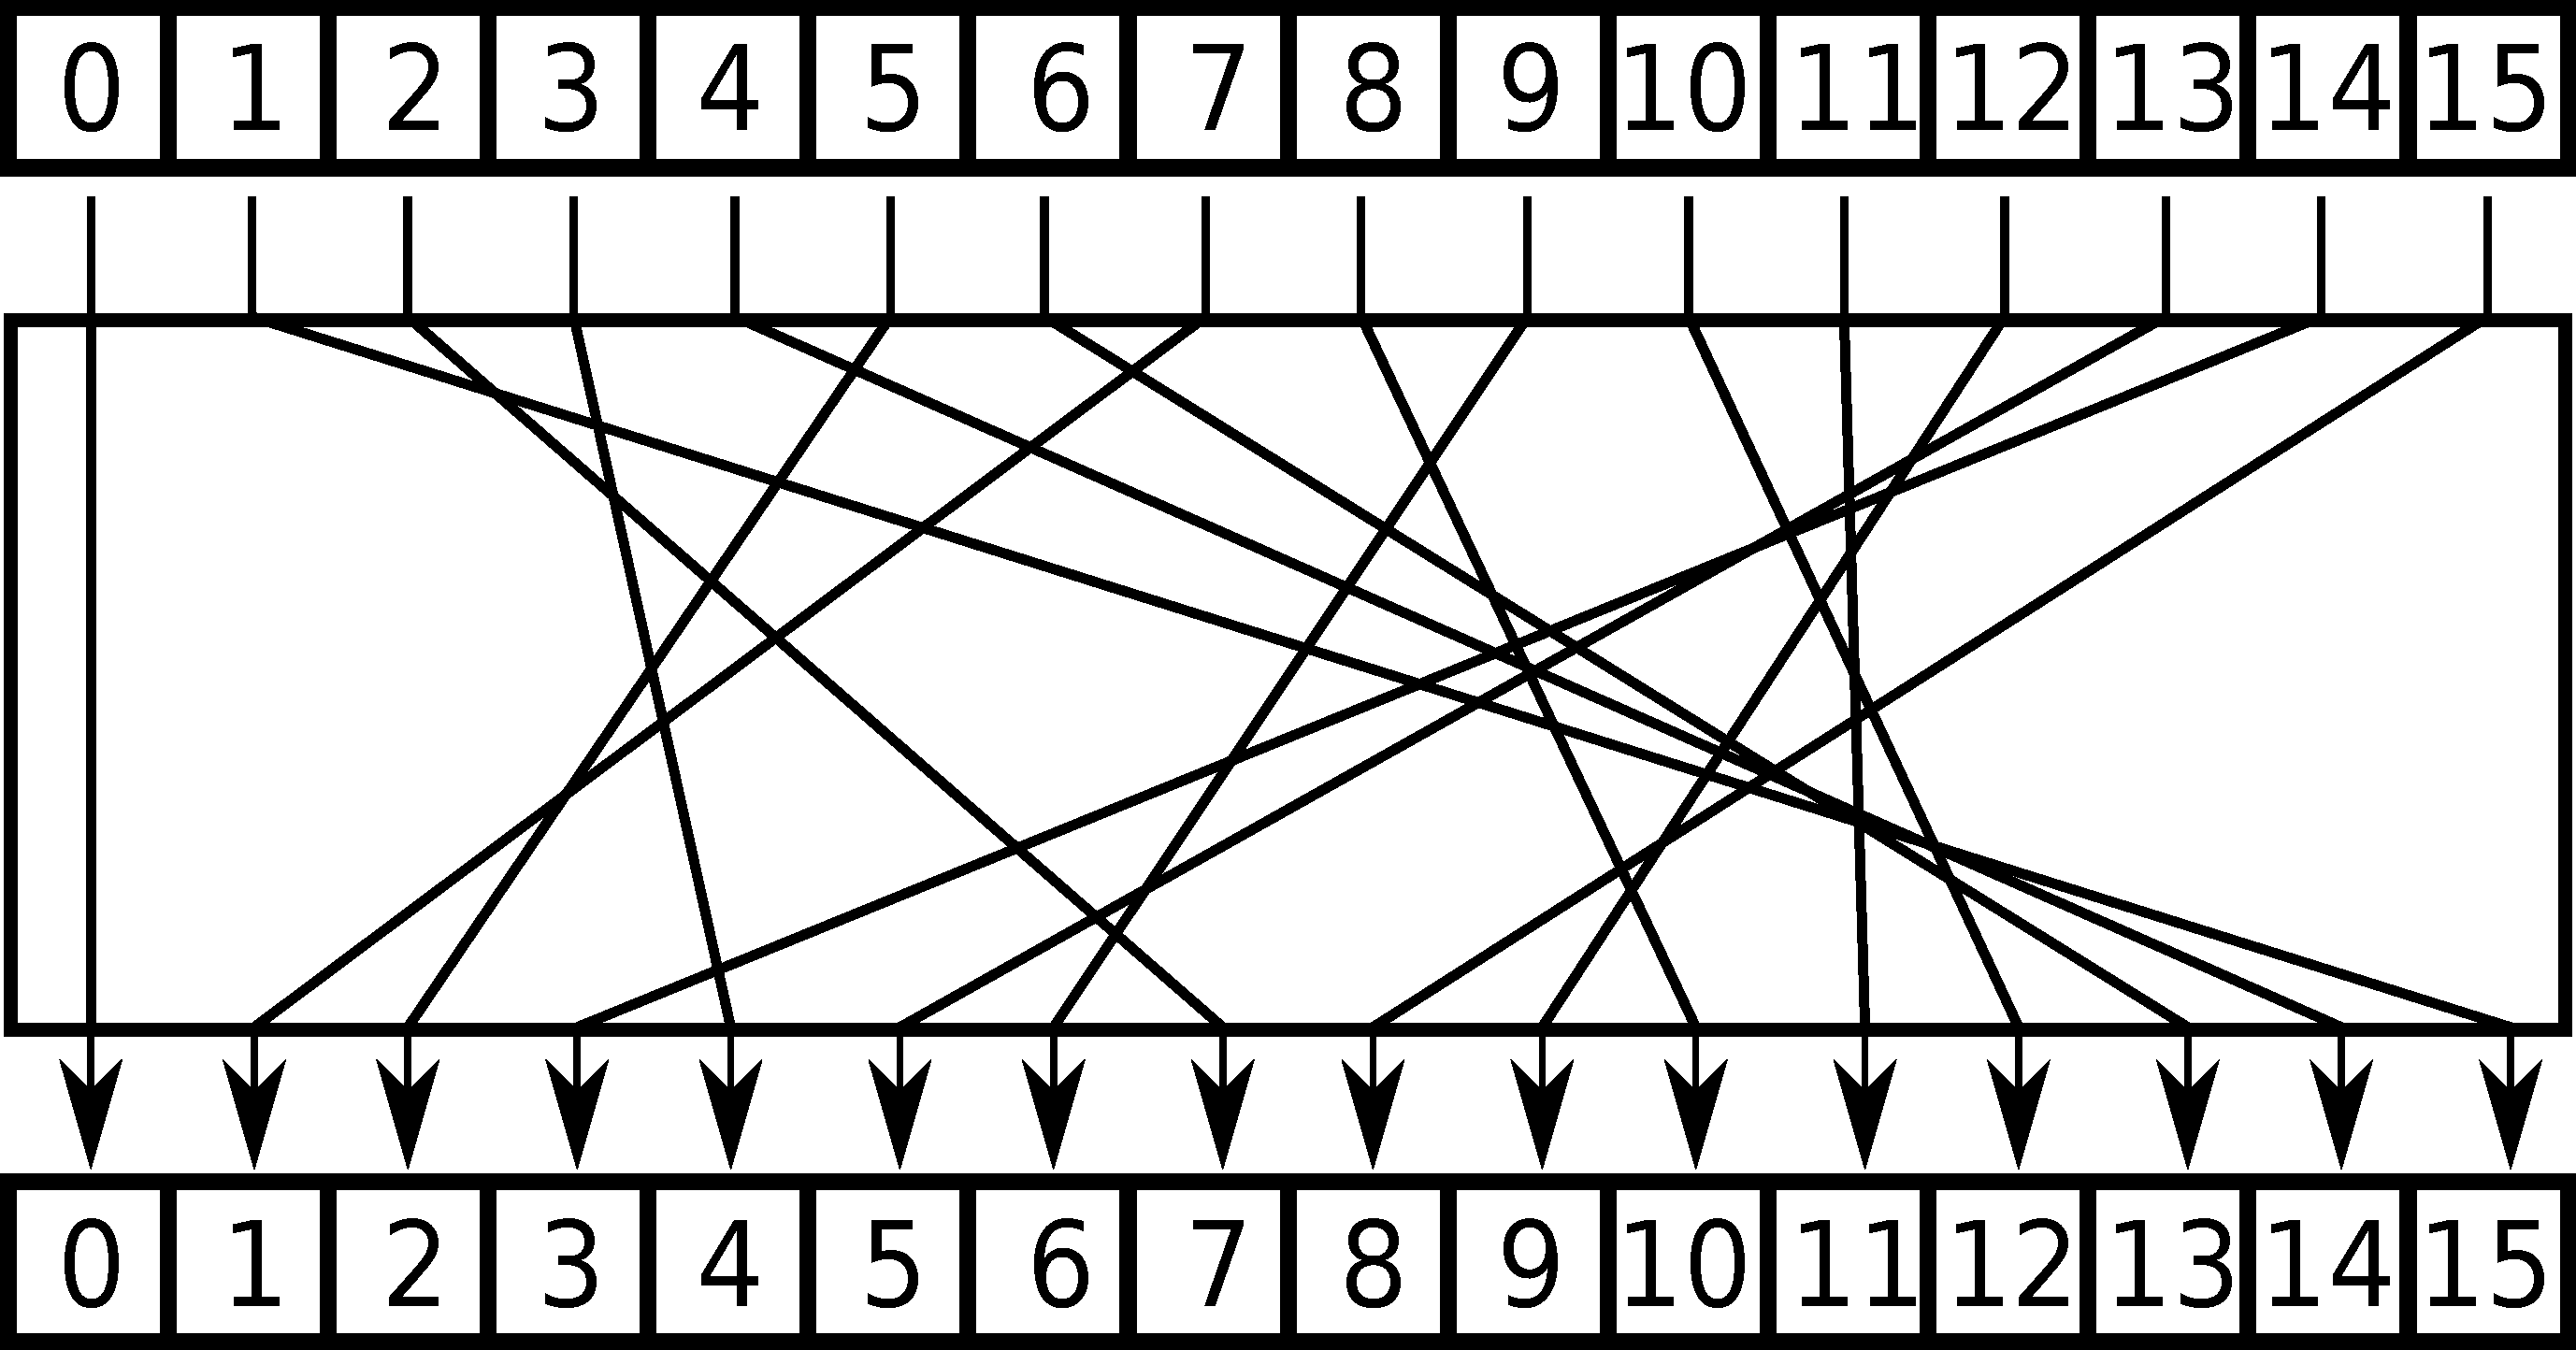
\includegraphics[scale=0.25]{imgs/diagram.pdf}
    \end{center}
    % \legend{Fonte: \citeonline[p. 24]{araujo2012}}
\end{figure}

% ----------------------------------------------------------
% Questão 3
% ----------------------------------------------------------
\subsection*{\textbf{3.10 - Compute the bits number 1, 16, 33, and 48 at the output of the first round of the DES decryption, assuming that the ciphertext block is composed of all ones and the external key is composed of all ones.}}
\addcontentsline{toc}{subsection}{Questão 3.10}

\begin{Verbatim}[commandchars=\\\{\}, fontsize=\footnotesize]
Texto cifrado (64bits) = C: 1111 1111 1111 1111 1111 1111 1111 1111
                            1111 1111 1111 1111 1111 1111 1111 1111

Como a chave é composta apenas de 1's não sofrerá alterações ao longo das rodadas.
K\textsubscript{1}, K\textsubscript{2}, ..., K\textsubscript{n}:         1111 1111 1111 1111 1111 1111 1111
                        1111 1111 1111 1111 1111 1111 1111

Como o texto cifrado é composto apenas de 1's.
LD\textsubscript{0}RD\textsubscript{0} = IP(C) = SWAP32bits(IP(C))

LD\textsubscript{0}: 1111 1111 1111 1111 1111 1111 1111 1111
RD\textsubscript{0}: 1111 1111 1111 1111 1111 1111 1111 1111

LD\textsubscript{1} = RD\textsubscript{0}: 1111 1111 1111 1111 1111 1111 1111 1111

E/P(RD\textsubscript{0}) = 1111 1111 1111 1111 1111 1111
           1111 1111 1111 1111 1111 1111

E/P(RD\textsubscript{0}) xor K\textsubscript{16} = A: 0000 0000 0000 0000 0000 0000
                     0000 0000 0000 0000 0000 0000

A: 000000 000000 000000 000000 000000 000000 000000 000000

S\textsubscript{1}: (0,0) = 14\textsubscript{10} = 1110\textsubscript{2}
S\textsubscript{2}: (0,0) = 15\textsubscript{10} = 1111\textsubscript{2}
S\textsubscript{3}: (0,0) = 10\textsubscript{10} = 1010\textsubscript{2}
S\textsubscript{4}: (0,0) = 07\textsubscript{10} = 0111\textsubscript{2}
S\textsubscript{5}: (0,0) = 02\textsubscript{10} = 0010\textsubscript{2}
S\textsubscript{6}: (0,0) = 12\textsubscript{10} = 1100\textsubscript{2}
S\textsubscript{7}: (0,0) = 04\textsubscript{10} = 0100\textsubscript{2}
S\textsubscript{8}: (0,0) = 13\textsubscript{10} = 1101\textsubscript{2}

B: 1110 1111 1010 0111 0010 1100 0100 1101

P(B):         1101 1000 1101 1000 1101 1011 1011 1100
LD\textsubscript{0}:          1111 1111 1111 1111 1111 1111 1111 1111
P(B) xor LD\textsubscript{0}: 0010 0111 0010 0111 0010 0100 0100 0011
RD\textsubscript{1}:          0010 0111 0010 0111 0010 0100 0100 0011

LD\textsubscript{1} || RD\textsubscript{1}: 1111 1111 1111 1111 1111 1111 1111 1111 
            0010 0111 0010 0111 0010 0100 0100 0011

Output of the first round: 
BIT 01 = 1  
BIT 16 = 1
BIT 33 = 0
BIT 48 = 1
\end{Verbatim}

% ----------------------------------------------------------
% Questão 4
% ----------------------------------------------------------
\subsection*{\textbf{3.11 - This problem provides a numerical example of encryption using a one-round version of DES. We start with the same bit pattern for the key K and the plaintext, namely:}}
\addcontentsline{toc}{subsection}{Questão 3.11}
\begin{Verbatim}
Hexadecimal notation:  0 1 2 3 4 5 6 7 8 9 A B C D E F

Binary notation:       0000 0001 0010 0011 0100 0101 0110 0111
                       1000 1001 1010 1011 1100 1101 1110 1111
\end{Verbatim}
\subsubsection*{\textbf{a. Derive K\textsubscript{1}, the first-round subkey.}}

\begin{Verbatim}[commandchars=\\\{\}, fontsize=\footnotesize]

PC-1:       1111000011001100101010100000 1010101011001100111100000000
LS:         1110000110011001010101000001 0101010110011001111000000001

PC-2 = K\textsubscript{1}:  0000 1011 0000 0010 0110 0111 
            1001 1011 0100 1001 1010 0101

\end{Verbatim}

\subsubsection*{\textbf{b. Derive L\textsubscript{0}, R\textsubscript{0}.}}

\begin{Verbatim}[commandchars=\\\{\}, fontsize=\footnotesize]
IP: 11001100000000001100110011111111 11110000101010101111000010101010

L\textsubscript{0}: 1100 1100 0000 0000 1100 1100 1111 1111
R\textsubscript{0}: 1111 0000 1010 1010 1111 0000 1010 1010
\end{Verbatim}


\subsubsection*{\textbf{c. Expand R\textsubscript{0} to get E[R\textsubscript{0}], where E[\#] is the expansion function of Table S.1.}}

\begin{Verbatim}[commandchars=\\\{\}, fontsize=\footnotesize]
R\textsubscript{0}:     1111   0000   1010   1010   1111   0000   1010   1010
E[R\textsubscript{0}]: 011110 100001 010101 010101 011110 100001 010101 010101
\end{Verbatim}

\subsubsection*{\textbf{d. Calculate A = E[R\textsubscript{0}] $\oplus$ K\textsubscript{1}.}}

\begin{Verbatim}[commandchars=\\\{\}, fontsize=\footnotesize]
K\textsubscript{1}:                 0000 1011 0000 0010 0110 0111 1001 1011 0100 1001 1010 0101
E[R\textsubscript{0}]:              0111 1010 0001 0101 0101 0101 0111 1010 0001 0101 0101 0101
A = E[R\textsubscript{0}] xor [K\textsubscript{1}]: 0111 0001 0001 0111 0011 0010 1110 0001 0101 1100 1111 0000
\end{Verbatim}

\subsubsection*{\textbf{e. Group the 48-bit result of (d) into sets of 6 bits and evaluate the corresponding S-box substitutions.}}

\begin{Verbatim}[commandchars=\\\{\}, fontsize=\footnotesize]
A: 011100 010001 011100 110010 111000 010101 110011 110000

S\textsubscript{1}: (0,14) = 00\textsubscript{10} = 0000\textsubscript{2}
S\textsubscript{2}: (1,08) = 12\textsubscript{10} = 1100\textsubscript{2}
S\textsubscript{3}: (0,14) = 02\textsubscript{10} = 0010\textsubscript{2}
S\textsubscript{4}: (2,09) = 01\textsubscript{10} = 0001\textsubscript{2}
S\textsubscript{5}: (2,12) = 06\textsubscript{10} = 0110\textsubscript{2}
S\textsubscript{6}: (1,10) = 13\textsubscript{10} = 1101\textsubscript{2}
S\textsubscript{7}: (3,09) = 05\textsubscript{10} = 0101\textsubscript{2}
S\textsubscript{8}: (2,08) = 00\textsubscript{10} = 0000\textsubscript{2}

\end{Verbatim}

\subsubsection*{\textbf{f. Concatenate the results of (e) to get a 32-bit result, B.}}

\begin{Verbatim}[commandchars=\\\{\}, fontsize=\footnotesize]
B: 0000 1100 0010 0001 0110 1101 0101 0000
\end{Verbatim}

\subsubsection*{\textbf{g. Apply the permutation to get P(B).}}

\begin{Verbatim}[commandchars=\\\{\}, fontsize=\footnotesize]
P(B): 1001 0010 0001 1100 0010 0000 1001 1100
\end{Verbatim}

\subsubsection*{\textbf{h. Calculate R\textsubscript{1} = P(B) $\oplus$ L\textsubscript{0}.}}

\begin{Verbatim}[commandchars=\\\{\}, fontsize=\footnotesize]
P(B): 1001 0010 0001 1100 0010 0000 1001 1100
L\textsubscript{0}:   1100 1100 0000 0000 1100 1100 1111 1111
R\textsubscript{1}:   0101 1110 0001 1100 1110 1100 0110 0011
\end{Verbatim}

\subsubsection*{\textbf{i. Write down the ciphertext.}}

\begin{Verbatim}[commandchars=\\\{\}, fontsize=\footnotesize]
L\textsubscript{1} = R\textsubscript{0}: 1111 0000 1010 1010 1111 0000 1010 1010
R\textsubscript{1} = R\textsubscript{0}: 0101 1110 0001 1100 1110 1100 0110 0011

Ciphertext = L\textsubscript{1} || R\textsubscript{1} : 1111 0000 1010 1010 1111 0000 1010 1010
                        0101 1110 0001 1100 1110 1100 0110 0011

Obs.: Como foi utilizado apenas uma rodada, não utilizei o swap de 32
      bits e a permutação por IP\textsuperscript{-1}.
\end{Verbatim}

% ----------------------------------------------------------
% Questão 5
% ----------------------------------------------------------
\subsection*{\textbf{3.12 - Compare the initial permutation table (Table S.1a) with the permuted choice one table (Table S.3b). Are the structures similar? If so, describe the similarities. What conclusions can you draw from this analysis?}}
\addcontentsline{toc}{subsection}{Questão 3.12}

Comparando a IP com a PC-1 pode se observar que suas estruturas são similares, a grande diferença de uma para a outra é a remoção dos 8 bits a seguir: 64 56 48 40 32 24 16 08, que não estão presentes na PC-1, os bits restantes estão presentes em ambas as tabelas. Conforme analisado, essas tabelas de permutações não aparentam contribuir para a segurança criptográfica do algoritmo.



% ----------------------------------------------------------
% Questão 6
% ----------------------------------------------------------
\subsection*{\textbf{3.16 - Refer to Figure G.2, which depicts key generation for S-DES.}}
\addcontentsline{toc}{subsection}{Questão 3.16}
\subsubsection*{\textbf{a. How important is the initial P10 permutation function?}}

A permutação P10 é uma permutação simples de um para um, ou seja, é apenas um rearranjo da chave K. Logo, a saída da P10 assim como a chave K permitem 2\textsuperscript{10} possibilidades de chaves únicas, com isso, a permutação P10 é indiferente para segurança do algoritmo.  

\subsubsection*{\textbf{b. How important are the two LS-1 shift functions?}}

Assim como a permutação P10 a LS-1 é apenas um rearranjo da ordem dos bits, e o número de possibilidades de chaves únicas mantém-se inalterado (2\textsuperscript{10} possibilidades). Logo, ela não adiciona em nada para a segurança do algoritmo.


% ----------------------------------------------------------
% Questão 7
% ----------------------------------------------------------
\subsection*{\textbf{3.18 - Using S-DES, decrypt the string (10100010) using the key (0111111101) by hand. Show intermediate results after each function (IP,F\textsubscript{K},SW,F\textsubscript{K},IP\textsuperscript{-1}). Then decode the first 4 bits of the plaintext string to a letter and the second 4 bits to another letter where we encode A through P in base 2 (i.e., A = 0000, B = 0001, ..., P = 1111). \textit{Hint}: As a midway check, after the application of SW, the string should be (00010011).}}
\addcontentsline{toc}{subsection}{Questão 3.18}

\begin{Verbatim}[commandchars=\\\{\}, fontsize=\footnotesize]

        Key:                 01111 11101
        P10:                 11111 10011
        First  5bits LS-1:   11111
        Second 5bits LS-1:         00111
        K1(8bits) after P8:   0101 1111
        First 5bits LS-2:    11111 
        Second 5bits LS-2:         11100
        K2(8bits) after P8:   1111 1100

        Ciphertext:           1010 0010
        \underline{IP:                   0011 0001}

        Fk Start:
        E/P:                  1000 0010  
        E/P xor K2:           0111 1110
        Box S0:                 00
        Box S1:                    00
        P4:                     00 00
        P4 xor IP(First 4bits): 00 11
        \underline{Fk Out:               0011 0001}

        \underline{SW:                   0001 0011}

        Fk Start:
        E/P:                  1001 0110  
        E/P xor K1:           1100 1001
        Box S0:                 01
        Box S1:                    10
        P4:                     10 10 
        P4 xor SW(First 4bits): 10 11 
        \underline{Fk Out:               1011 0011}
        \underline{IP-1:                 1110 1010}
        \underline{Plaintext:            OK}
\end{Verbatim}

% ---
% Finaliza a parte no bookmark do PDF, para que se inicie o bookmark na raiz
% ---
\bookmarksetup{startatroot}% 
% ---

% ---
% Conclusão
% ---
% \section*{Considerações finais}
% \addcontentsline{toc}{section}{Considerações finais}

% ----------------------------------------------------------
% ELEMENTOS PÓS-TEXTUAIS
% ----------------------------------------------------------
\postextual

% ----------------------------------------------------------
% Referências bibliográficas
% ----------------------------------------------------------
\nocite{Stallings:2010:CNS:1824151}
\bibliography{bibliography}

\end{document}